\chapter{深度神经网络模型的设计}
\section{引言}

在我们的项目中,最终缺陷的表现并非是传统的分类,我们最后需要对图像进行标记,为此我们需要在预测缺陷类型的同时,将缺陷用边框标注出来进行分类。

我们选取了基于\cite{DBLP:journals/corr/abs-1904-08900}的CornerNet-Lite网络进行修改,CornerNet-Lite是是CornerNet网络的两种有效变体的组合,在此基础上提高了精度和效率。

\section{模型网络结构}

CornerNet的核心在于相对于传统的基于中心的anchor boxes思路,因为左上角和右下角的一对定点。 

\subsection{特征提取模块的设计}
\subsubsection{网络设计}

Hourglass模块网络是\cite{DBLP:journals/corr/NewellYD16}中提出的一种网络结构,其堆叠在一起,呈现出一种沙漏的结构,能够展现出图像所有尺度中的信息。

Hourglass模块由一系列对称的重复结构组成,首先是降低分辨率的池化操作,接着是提升分辨率的上采样过程,池化和上采样的结合能够保留各个尺度的信息,下面图\ref{fig:hourglass}显示出了Hourglass模块的特征。

但是因为下采样会损失信息,最终的上采样信息并不能完全还原我们图像信息,而我们在预测局部的时候只需要局部信息,整体的时候又只需要整体信息,我们最终结果不能忍受信息的缺失,因此我们引入了残差模块,通过pipeline来处理不同尺度的信息,残差模块能够将前期未下采样的图像信息传递到后期的对应分辨率图像中,借以保存原本的空间信息。


\begin{figure}[!tbp]
    \centering
    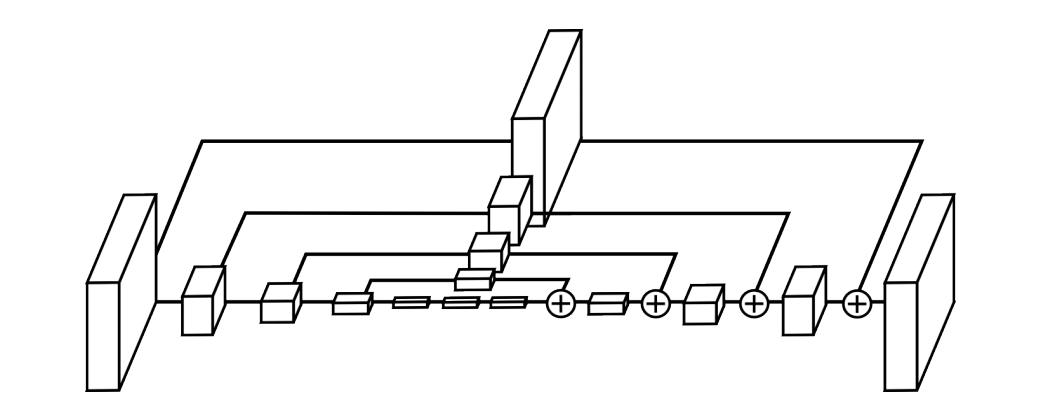
\includegraphics[width=\textwidth]{figures/hourglass.png}
    \caption{Hourgalss模块图\cite{newell2016stacked}}
    \vspace{-1em}
    \label{fig:hourglass}
\end{figure}

图像经过了Hourglass模块的数次池化、卷积的操作后分辨率降低,并在每个最大池化之前分出一个分支使用更多的卷积以提取更多的特征,在之后的上采样过程后,和之前的特征集相加获取这个尺度的总体特征。

图像在上采样回到我们指定的分辨率后,最终再通过两个尺度为 $ 1 \times 1 $ 的卷积层进行预测。

我们的输入图像是 $ 512 \times 512 $ 的尺寸,我们经过尺度为 $ 7 \times 7 $ 的卷积核处理后,将分辨率降低4倍。 我们设置了并联的Hourglass模块,将图像进行下采样和上采样,让最终的输出分辨率不变。

再之后我们将分为两部分,分别去预测两个box的边角,及左上角和右下角的点。称其为Corner pooling。角池化的运用会返回三个参数。用于预测角点信息的热力图heatmap,是一个 $ C(ategory) \times H(eight) W(eight) $ 的特征张量,其值被归一化到了 $ [0,1] $ 之间,用以表示这个点在不同类别下面的预测的分数。用于对预测点做分组的embeddings,找到应该同属于一个目标的左上和右下点。以及用于对预测的框做微调用的offset数组。

于此我们已经有了对于预测角点的位置的张良heatmap,我们要确定我们的损失函数 $ L_det $,并由此来训练我们的模型,损失函数的定义是由下式子定义的:

\begin{eqnarray}
    L_{det} = -\frac{1}{N} \sum^{C}_{c=1}\sum^{H}_{i=1}\sum^{W}_{j=1} \left\{  
        \begin{array}{lr}  
        (1-p_{cij})^{\alpha}\log(p_cij), & y_{cij} == 1\\  
        (1-y_{cij})^{\beta}(p_{cij})^{\alpha}\log(1-p_{cij}) & y_{cij} != 1    
        \end{array}  
\right.  
\end{eqnarray}

$ y_{cij} $ 表示预测点是否是我们标签给出的点,如果是指定点即其为1,且预测点越接近我们的标签点则值越接近1,$ y_{cij} $ 的值我们使用高斯分布,用于实现性能更好的状态分布。并使用了heatmap中的归一化概率分布 $ p_{cij} $ 来实现最终的损失函数。我们对图像中所有点和所有通道进行遍历求和。对于一张图像上可能有的多个缺陷目标,损失函数肯定会相应变大,我们除去检测目标所带来的影响,取得平均值。

第二个返回的参数是embedding,我们需要将我们的预测点进行分组,embedding向量距离一般征兆着两点之间的关系,特别对于同一个缺陷目标来说,其左上角和右下角的预测点应该有较小的embedding向量值。

我们就使用两个损失函数去实现这个embedding的优化,其中一个是 $ L_{pull} $,即我们需要使用这个来拉近同一个对象的对点距离

\begin{eqnarray}
    L_{pull} = \frac{1}{N}\sum^{N}_{k=1}[(e_{tk}-e_k)^2+(e_{bk}-e_k)^2]
\end{eqnarray}

另外一个是 $ L_{push} $ ,用来扩大不同目标的对点距离:

\begin{eqnarray}
    L_{push} = \frac{1}{N(N-1)}\sum^{N}_{k=1}\sum^{N}_{j=1,j\neq k} max(0,\triangle-\lvert e_k -e_j \rvert)
\end{eqnarray}


而第三个返回参数是offset的精度损失,用以表示由于下采样到上采样后的精度偏差,因为下采样并非一定能够完全取到2的倍数,下采样过程中可能导致图像的移位,对小尺度的缺陷目标有精度损失,增加回归算法的准确性。这个误差也应该我们尽量减小。为此我们有第三个损失函数:

\begin{eqnarray}
    L_{off} = \frac{1}{N}\sum^{N}_{k=1}Smooth_{L1}Loss(o_k,\hat{o_k})
\end{eqnarray}

其中 $ o_k $ 的定义为损失的精度信息:

\begin{eqnarray}
    o_k = (\frac{x_k}{n}-\lfloor\frac{x_k}{n}\rfloor,\frac{y_k}{n}-\lfloor\frac{y_k}{n}\rfloor)
\end{eqnarray}

而 $ Smooth_{L1}Loss $ 是:

\begin{eqnarray}
    Smooth_{L1}(x) = 
    \left\{  
        \begin{array}{lr}  
        \frac{1}{2}x^2, & \lvert x \rvert \le 1\\  
        \lvert x \rvert - 0.5 & \lvert x \rvert \geq 1    
        \end{array}  
\right.  
\end{eqnarray}

在确定了预测的corner点之后,我们引入了corner pooling的角池化操作,我们要训练就需要图像的信息,明显的,左上角点下方有图像左侧信息,而左上角右边有图像顶端信息,则我们通过corner pooling就能够同时获得图像的两个方面的信息。而最终的算式是将此点与下方和右方的所有点的最大值相加得到此点的角池化值。

我们引入了SqueezeNet的理念,可以更利于小型化和分布式训练,我们将原本的残差模块更改为fire模块,使用 $ 1 \times 1$的卷积核的squeeze层替代,并在之后使用 $ 1 \times 1 + 3\times 3 $ 卷积核的混合层。

为了增加准确性,我们再对fire module进行了改进,在file模块中第二层本来使用包括 $ 3 \times 3 $ 卷积核的混合层,我们假设出如果这些通道之间互不相关,我们就可以就能进行退耦合,将卷积层的各个通道分开映射。做成深度可分离的卷积Xception。

这样能大量降低计算量,对于输入图 $ H(eight) \times W(width) \times I_C(ategory) $ ,输出图 $ H(eight) \times W(width) \times O_C(ategory) $,和卷积核 $ K \times K $ 来说,使用深度可分离卷积能够将计算量从传统的:

\begin{eqnarray}
    H(eight) \times W(width) \times I_C(ategory) \times O_C(ategory) \times K \times K
\end{eqnarray}

转换成我们现在的:

\begin{eqnarray}
    H \times W \times I_C \times K \times K + I_C \times O_C \times H \times W
\end{eqnarray}

\section{本章总结}

本章叙述了我们用于缺陷识别的网络结构,CornerNet-lite的网络结构最主要的是靠两个串联的Hourglass沙漏型模块组成的,通过在不同尺度上的offset数组,获取在不同尺度下的精度偏差。通过角池化操作获得我们所需要的图像的边信息。并在实现惨差模块时使用了fire module用以旁路卷积时使用更小的卷积核替代,用以降低运算量。对于不同通道我们进行分离后卷积操作,能再一次降低我们的运算复杂度。通过这几步,我们去最小化我们的损失函数后就能获取到缺陷对象的边界点了。